<<<<<<< HEAD
% --------------------------------------
% Document Class
% --------------------------------------
\documentclass[a4paper,11pt]{article}
% --------------------------------------



% --------------------------------------
% Use Package
% --------------------------------------


\usepackage[francais]{babel}
%\usepackage{ucs}
\usepackage[utf8]{inputenc}
\usepackage[T1]{fontenc}

\usepackage{makeidx}
\usepackage{color}
\usepackage{graphicx}
\usepackage{float}
\usepackage[hidelinks]{hyperref} 
\usepackage{geometry}
%\usepackage{lastpage}
%\usepackage{marginnote}
\usepackage{fancyhdr}
%\usepackage{titlesec}
%\usepackage{framed}
\usepackage{amsmath}
\usepackage{empheq}
\usepackage{array}
\usepackage{multicol}
\usepackage{csquotes}
%\usepackage{adjustbox}

% insert code
\usepackage{listings}

% define our color
\usepackage{xcolor}

% code color
\definecolor{ligthyellow}{RGB}{250,247,220}
\definecolor{darkblue}{RGB}{5,10,85}
\definecolor{ligthblue}{RGB}{1,147,128}
\definecolor{darkgreen}{RGB}{8,120,51}
\definecolor{darkred}{RGB}{160,0,0}

% other color
\definecolor{ivi}{RGB}{141,107,185}


\lstset{
    language=java,
    captionpos=b,
    extendedchars=true,
    frame=lines,
    numbers=left,
    numberstyle=\tiny,
    numbersep=5pt,
    keepspaces=true,
    breaklines=true,
    showspaces=false,
    showstringspaces=false,
    breakatwhitespace=false,
    stepnumber=1,
    showtabs=false,
    tabsize=3,
    basicstyle=\small\ttfamily,
    backgroundcolor=\color{ligthyellow},
    keywordstyle=\color{ligthblue},
    morekeywords={include, printf, uchar},
    identifierstyle=\color{darkblue},
    commentstyle=\color{darkgreen},
    stringstyle=\color{darkred},
}


% --------------------------------------



% --------------------------------------
% Page setting
% --------------------------------------
%\pagestyle{empty}
\setlength{\headheight}{15pt}

\setcounter{secnumdepth}{3}
\setcounter{tocdepth}{2}

\makeatletter
\@addtoreset{chapter}{part}
\makeatother 

\hypersetup{         % parametrage des hyperliens
  colorlinks=true,      % colorise les liens
  breaklinks=true,      % permet les retours à la ligne pour les liens trop longs
  urlcolor= blue,       % couleur des hyperliens
  linkcolor= black,     % couleur des liens internes aux documents (index, figures, tableaux, equations,...)
  citecolor= green      % couleur des liens vers les references bibliographiques
}

% --------------------------------------

% --------------------------------------
% Information
% --------------------------------------
\title{Compte-rendu TP10 TI : Détection de contours par approches du second ordre}
\author{Elliot VANEGUE et Gaëtan DEFLANDRE}
% --------------------------------------

\definecolor{myColor}{rgb}{0.5, 0.1, 0.75}

% --------------------------------------
% Begin content
% --------------------------------------
\begin{document}

% Set language to english
  \selectlanguage{francais}

  % Start the page counting
  \pagenumbering{arabic}

  \maketitle
  
  \mbox{}
  \newpage
  \clearpage
  
  \section*{Introduction}
   Lors du TP précédent, nous avons pu voir la détection de contours par approche du premier ordre. Nous avons
   calculé la dérivé de l'image afin de récupérer la norme et la direction du gradient de chaque pixel. Dans ce TP
   nous allons utiliser une approche du second ordre avec le calcul du Laplacien, puis nous effectuerons un seuillage
   des passages par zéro.

  \section{Calcul du Laplacien}
  Nous allons dans un premier temps appliquer un masque de convolution. Ce masque est un masque normalisé
  qui est le résultat de la dérivé second directionnelle. Lorsque nous l'appliquons à l'image des spores, nous
  voyons qu'il fait plus ou moins ressortir les contours de l'image.\\
  
  \begin{center}
  \begin{tabular}{|c|c|}
   \hline
   masque appliqué & résultat\\
   \hline
   $\begin{pmatrix} 0 & 1 & 0\\ 1 & -4 & 1\\ 0 & 1 & 0 \end{pmatrix}$ & 
\includegraphics[width=3cm]{../convolution0.png}\\
   \hline
   $\begin{pmatrix} 1 & 0 & 1\\ 0 & -4 & 0\\ 1 & 0 & 1 \end{pmatrix}$ & 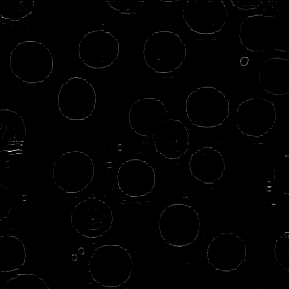
\includegraphics[width=3cm]{../convolution1.png}\\
   \hline
   $\begin{pmatrix} 1 & 4 & 1\\ 4 & -20 & 4\\ 1 & 4 & 1 \end{pmatrix}$ & 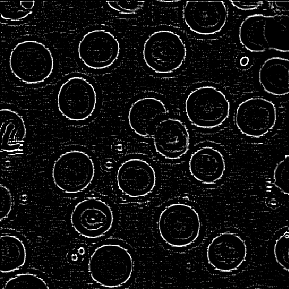
\includegraphics[width=3cm]{../convolution4.png}\\
   \hline
  \end{tabular}
  \end{center}

  Comme on peut le voir sur les résultats, plus le centre du masque est petit et plus les contours de l'image ressorte. 
  Cependant, le résultat n'en est pas forcément meilleur, car plus les contours sont visibles et plus du bruit apparaît.
  Cela se voit particulièrement bien lorsque nous mettons en évidence les pixels mis à zéro par le Laplacien.
  
  \begin{figure}[H]
   \center
   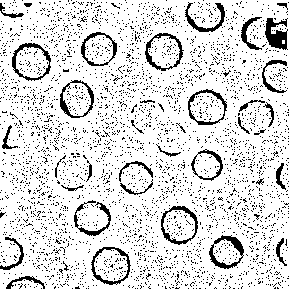
\includegraphics[width=5cm]{../laplacien0.png}
   \caption{Mise en évidence des pixels mis à zéro par le Laplacien}
  \end{figure}

  On voit clairement qu'une approche du second ordre fait ressortire les contours, mais également beaucoup de bruit. 
  Pour minimiser ce problème nous allons effectuer un seuillage des passages par zéro du Laplacien.
  
  \section{Seuillage des passages par 0 du Laplacien}
  Pour effectuer ce seuillage, nous utilisons un seuil déterminé par l'utilisateur et l'image que nous avons
  calculé grâce au masque du Laplacien. Pour déterminé si un pixel fait parti d'une contour nous parcourons l'ensemble de l'image 
  et nous vérifions le voisinage de chaque pixel. Si le voisinage du pixel traité répond aux conditions suivantes : $max > seuil$ et $min < -seuil$
  alors le pixel fait partie d'un contour. Cela permet d'éliminer les fréquences trop basse de l'image.\\ 
  
  Avec cette méthodologie, nous utilisons un seuil de 24 pour l'image des spores avec le premier masque du tableau précédent, ce qui nous donne un résultat relativement
  satisfaisant. Au delà de ce seuil, les contours des spores sont de plus en plus imcomplet. Et en dessous de ce seuil, le bruit est
  trop important.
  
  \begin{figure}[H]
   \center
   
\includegraphics[width=5cm]{../seuillage24.png}
   \caption{Seuillage de l'image des spores avec un seuil de 24}
  \end{figure}
  
  On ne peut donc pas obtenir des contours complets avec un minimum de bruit avec cette méthode. Pour résoudre ce problème
  nous allons utilise le filtre LoG\footnote{Laplacian of Gaussian}.
  
  \section{Utilisation du filtre LoG et détection multi-échelles}
  Le filtre LoG va permettre de lisser l'image avec un noyau gaussien dont l'écart type de la courbe gaussienne est défini par
  sigma. Pour que ce masque soit efficace il faut que sa taille soit adapté au sigma et que cette taille soit impaire. Nous prenons
  donc comme taille de masque $7*sigma$.\\
  %TODO
  %Nous pouvons alors calculer le seuil avec la formule
  %TODO voir approche multi echelle
  
  Nous allons maintenant utiliser la norme du gradient pour seuiller l'image que nous avons calculer.
\end{document}  